\subsection{Architecture}
Informer (\citet{https://doi.org/10.48550/arxiv.2012.07436}) leverages the non-autoregressive decoding (termed \textit{generative inference} in the paper) for time series forecasting. 
The main idea is to predict $L_\text{target}$ future timestamps in just one forward pass. 
The model also develops an asymptotically efficient attention mechanism called ProbSparse attention, although we empirically show that it performs no better than vanilla attention in terms of speed and accuracy. 
Therefore, in this section, we focus on vanilla multihead attention (\citet{https://doi.org/10.48550/arxiv.1706.03762}) with different decoding schemes. 

\subsubsection{Non-Autoregressive Decoder}
The autoregressive decoder follows the design of seq2seq Transformer models. 
In a long sequence forecasting setting, when predicting values $X_{j, *} \in \Rb^{d}$ at timestamp $j$, we concatenate all previous predictions $\hat{\Xv}_{<j, *} \in \Rb^{(j - 1) \times d}$ and feed them into the model.  
Notice that this decoding scheme is inherently sequential and hence can be extremely slow during inference. 
Moreover, the model is vulnerable to the training-testing distribution shift due to teacher-forced training (\citet{6795228}). 

On the other hand, non-autoregressive decoder forecasts in parallel. 
The layout of decoder input is shown in Figure \ref{fig:nonauto_input}, where the dark green blocks are (optionally) previous observations that create \textit{context} for decoding, 
the white zero blocks are placeholders where predictions will be made, 
and the light green blocks are positional and temporal embeddings which are intact. 
Finally, a triangular causal mask is applied to decoder's self attention module so that each timestamp can attend to previous observations only. 

\begin{figure}
    \centering
    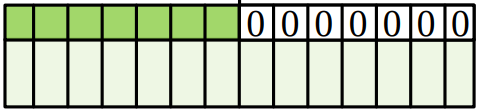
\includegraphics[width=0.3\textwidth]{img/nonauto_input.png}
    \caption{Input to a non-autoregressive decoder.}
    \label{fig:nonauto_input}
\end{figure}

\subsubsection{ProbSparse Attention Module}
For each head of a vanilla multihead attention module, the output is computed by $$\text{Attention}(\Qv, \Kv, \Vv) = \text{softmax}(\frac{\Qv\Kv^T}{\sqrt{d}}) \Vv.$$
Overall, the output is $\text{Multihead}(\Qv, \Kv, \Vv) = [\text{head}_1 \| \text{head}_2 \| \cdots \| \text{head}_h]\Wv^O$, where we define $\text{head}_i = \text{Attention}(\Qv\Wv_i^Q, \Kv\Wv_i^K, \Vv\Wv_i^V)$. 
Here, $\|$ is the concatenation operator and $\Wv$'s are projection matrices of appropriate shapes. 

ProbSparse attention assumes the sparicty in the query signal and only select a sparse subset of tokens $\overline{\Qv}$ to compute $\text{Multihead}(\overline{\Qv}, \Kv, \Vv)$. 
More details can be found in the Informer's paper. 
However, as noted previously we only use vanilla attention to perform analysis in this section. 

\subsection{Experiments}

While the Informer paper (\citet{https://doi.org/10.48550/arxiv.2012.07436}) does contain an ablation study on the non-autoregressive decoding, only two prediction lengths $L_\text{target}$ are examined and the authors did not decouple the influence of the noval attention module. 
To verify the superiority of a non-autoregressive decoder, we run more experiments on six real-world benchmarks and observe expected results. 

Interestingly, we notice that the decoder taking input as Figure \ref{fig:nonauto_input} is sufficient to perform forecasting. 
Therefore, we remove encoder and evaluate the \texttt{Decoder-Only} model as well. 

\subsubsection{Datasets}\label{benchmarks}

We use six real-world dataset that are popular in time series research community: \begin{itemize}
    \item \texttt{ETT}(\citet{https://doi.org/10.48550/arxiv.2012.07436}): This dataset is related to electric power deployment. The data is 7-dimensional plus a timestamp. 
    The sampling rate of \texttt{ETTh1} is 1 hour and of \texttt{ETTm2} is 15 minutes. 
    \texttt{ETTh1} has 14k observations in total, whereas \texttt{ETTm2} has 70k observations in total. 
    \item \texttt{Electricity}\footnote{https://archive.ics.uci.edu/ml/datasets/ElectricityLoadDiagrams20112014}: It contains electricity consumption of 321 clients. The sampling rate is 1 hour. There are 26k observations in total. 
    \item \texttt{Exchange}(\citet{https://doi.org/10.48550/arxiv.1703.07015}): It documents daily exchange rate across 7 countries. There are 8k observations in total. 
    \item \texttt{Traffic}\footnote{http://pems.dot.ca.gov/}: This is a collection of road occupancy rates of 862 San Francisco Bay area freeways. The sampling rate is 1 hour. There are 18k observations in total. 
    \item \texttt{Weather}\footnote{https://www.bgc-jena.mpg.de/wetter/}: This is local climatological data from 2010 to 2013 of the United States. The data is 20-dimensional plus a timestamp. 
    The sampling rate is 1 hour. There are 50k observations in total. 
    \item \texttt{ILI}\footnote{https://gis.cdc.gov/grasp/fluview/fluportaldashboard.html}: The dataset contains the percentage of patients with influenza-like illness from 2002 to 2021. 
    The data is 7-dimensional plus the timestamp with a 7-day sampling rate. There are 967 observations in total. 
\end{itemize}

\subsubsection{Results}
Figure \ref{fig:mse_nonauto} shows the mean square errors of forecasting results on different test datasets with varied prediction lengths. 
The lower the bar, the better the model. 
Overall, non-autoregressive decoding performs on par with, if not better than, autoregressive decoding. 
The gap is especially large in \texttt{Electricity} and \texttt{Traffic} datasets. 
A possible reason is that time series forecasting relies more on an understanding of large-scale pattern; 
instead, the dependencies on previous one timestamp or two are rather weak. 
Therefore, autoregression does not possess significant advantage. 

\begin{figure}
    \centering
    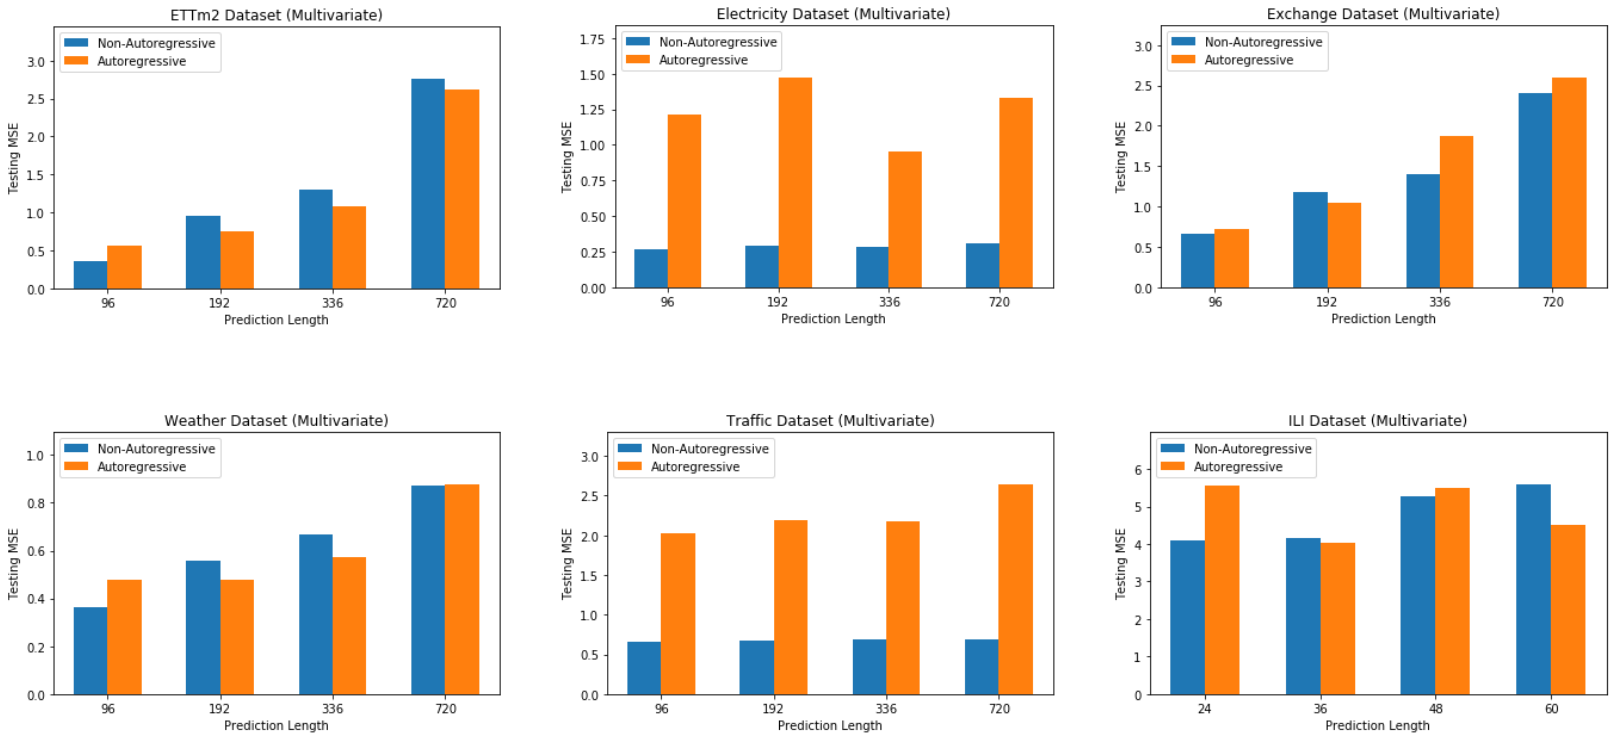
\includegraphics[width=\textwidth]{img/mse_nonauto.png}
    \caption{Mean square errors of autoregressive versus non-autoregressive decoding.}
    \label{fig:mse_nonauto}
\end{figure}

Taking the inference speed into account, Figure \ref{fig:nonauto_time} indicates that autoregressive decoding is an undisirable choice for sure. 
Interestingly, while \citet{https://doi.org/10.48550/arxiv.2012.07436} claims that Informer improves the asymptotic cost of the attention mechanism, empirically vanilla attention with non-autoregressive decoding takes even smaller amount of time. 
This result highlights the discrepancy between the asymptotic analysis and wall-clock time. 
Meanwhile, it reinforces the necessity of incorporating non-autoregressive decoding scheme into Transformer variants for the long sequence time series forecasting. 

\begin{figure}
    \centering
    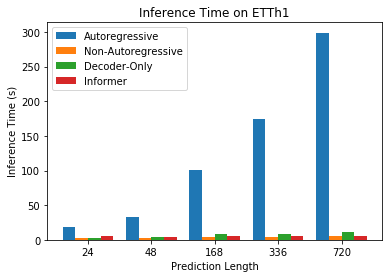
\includegraphics[width=0.5\textwidth]{img/nonauto_time.png}
    \caption{Inference speed measured by second on the \texttt{ETTh1} test dataset.}
    \label{fig:nonauto_time}
\end{figure}

As mentioned previously, we also evaluate a vanilla Transformer without an encoder, since the non-autoregressive decoder is theoretically with contextualized input (Figure \ref{fig:nonauto_input}) is sufficient in this setting. 
Figure \ref{fig:mse_noenc} compares results with state-of-the-art Transformer variants. 
Although the \texttt{Decoder-Only} model has achieved competitive performance against Informer, it falls short of more recent models equipped with the decomposition module. 
Moreover, we found empirically that \texttt{Decoder-Only} is insensitive as we scale up the model parameters. 
Thus, while removing the encoder can be a promising way to reduce model size robustly, it fails to generate significant improvement. 
The hope lies in the architecture innovation. 

\begin{figure}
    \centering
    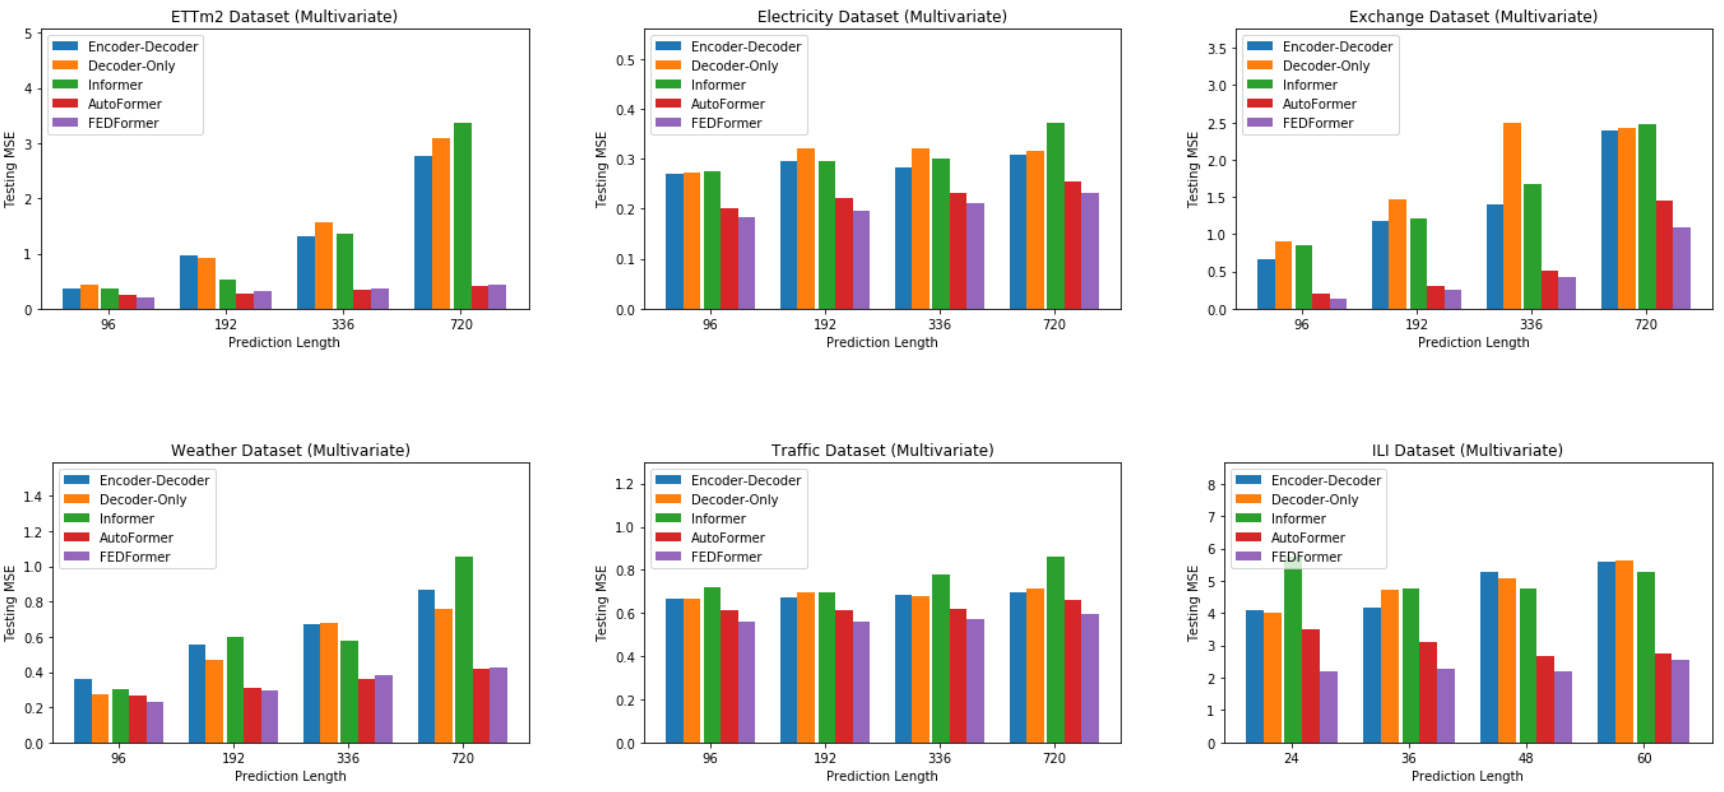
\includegraphics[width=\textwidth]{img/mse_noenc.png}
    \caption{Mean square errors of Transformers with and without encoder as well as state-of-the-art variants.}
    \label{fig:mse_noenc}
\end{figure}
